\chapter{Convolution}
\section{Examples}
\subsection{离散卷积的例子:丢骰子}
我有两枚骰子, 把这两枚骰子都抛出去, 求两枚骰子点数加起来为4的概率是多少?

这里问题的关键是,两个骰子加起来要等于4,这正是卷积的应用场景.
我们用 $f$ 表示第一枚骰子, $g$ 表示第二枚骰子, 有 $f(i) = g(i) = 1/6$.

两枚骰子加起来为4 的情况有:
$$(f * g)(4) = f(1)g(3) + f(2)g(2) + f(3)g(1) = \sum_{a + b = 4}f(a)g(b) = \sum_{m = 1}^3f(m)g(4 - m)$$

\subsection{连续卷积的例子:做馒头}
楼下早点铺子生意太好了,供不应求,就买了一台机器,不断的生产馒头.
假设馒头的生产速度是$f(t)$, 那么一天后生产出来的馒头总量为$$\int_0^{24} f(t)dt$$
馒头生产出来之后,就会慢慢腐败,假设腐败函数为$g(t)$ ,比如,$10$个馒头,$24$小时会腐败.
很容易推断出, 第一个小时生产出来的馒头, 一天后会经历24小时的腐败, 第二小时生产出来的馒头, 一天后会经历23小时的腐败.
如此, 我们可以知道, 一天后, 馒头总共腐败了:
$$\int_0^{24} f(t)g(24 - t)dt$$
这就是连续的卷积.

\subsection{矩阵的卷积}
$$
f =
\begin{bmatrix}
a_{00} & a_{01} & a_{02} \\
a_{10} & a_{11} & a_{12} \\
a_{20} & a_{21} & a_{22} \\
\end{bmatrix}
\et
g =
\begin{bmatrix}
b_{00} & b_{01} & b_{02} \\
b_{10} & b_{11} & b_{12} \\
b_{20} & b_{21} & b_{22} \\
\end{bmatrix}
$$

$f$ 和 $g$ 的卷积
$$
\begin{aligned}
c_{11}
& = (f * g)(2, 2) \\
& = a_{00}b_{22} + a_{01}b_{21} + a_{02}b_{20} + a_{10}b_{12} + a_{11}b_{11} + a_{12}b_{10} + a_{20}b_{02} + a_{21}b_{01} + a_{22}b_{00} \\
& = \sum_{i + j = 2 \et k + l = 2}a_{ik}b_{jl}
\end{aligned}
$$

\subsection{形象化的解释}
比如说你的老板命令你干活,你却到楼下打台球去了,后来被老板发现,他非常气愤,扇了你一巴掌(注意,这就是输入信号,脉冲),于是你的脸上会渐渐地(贱贱地)鼓起来一个包,
你的脸就是一个系统,而鼓起来的包就是你的脸对巴掌的响应,好,这样就和信号系统建立起来意义对应的联系.
下面还需要一些假设来保证论证的严谨:假定你的脸是线性时不变系统,也就是说,无论什么时候老板打你一巴掌,打在你脸的同一位置(这似乎要求你的脸足够光滑),
你的脸上总是会在相同的时间间隔内鼓起来一个相同高度的包来,并且假定以鼓起来的包的大小作为系统输出.好了,那么,下面可以进入核心内容-卷积了!

如果你每天都到地下去打台球,那么老板每天都要扇你一巴掌,不过当老板打你一巴掌后,你5分钟就消肿了,所以时间长了,你甚至就适应这种生活了.
如果有一天,老板忍无可忍,以$0.5$秒的间隔开始不间断的扇你的过程,这样问题就来了,第一次扇你鼓起来的包还没消肿,第二个巴掌就来了,你脸上的包就可能鼓起来两倍高,
老板不断扇你,脉冲不断作用在你脸上,效果不断叠加了,这样这些效果就可以求和了,结果就是你脸上的包的高度是随时间变化的一个函数了(注意理解),
如果老板再狠一点,频率越来越高,以至于你都辨别不清时间间隔了,那么,求和就变成积分了.

可以这样理解,在这个过程中的某一固定的时刻,你的脸上的包的鼓起程度和什么有关呢?
和之前每次打你都有关!但是各次的贡献是不一样的,越早打的巴掌,贡献越小,所以这就是说,
某一时刻的输出是之前很多次输入乘以各自的衰减系数之后的叠加而形成某一点的输出,然后再把不同时刻的输出点放在一起,形成一个函数,这就是卷积,
卷积之后的函数就是你脸上的包的大小随时间变化的函数.
本来你的包几分钟就可以消肿,可是如果连续打,几个小时也消不了肿了,这难道不是一种平滑过程么?
反映到公式上,f(a)就是第a个巴掌, g(x-a)就是第a个巴掌在x时刻的作用程度,乘起来再叠加就ok了,大家说是不是这个道理呢?
我想这个例子已经非常形象了,你对卷积有了更加具体深刻的了解了吗?

\section{Definition}
the convolution of $f$ and $g$, evluated at $c$ is defined:
$$(f\ast g)(c) = \sum_{a+b=c} f(a) \cdot g(b)$$
If we substitute $b = c − a$, we get:
$$(f\ast g)(c) = \sum_a f(a) \cdot g(c-a)$$
This is the standard definition of convolution.

如果$a, b, c$ 为vectors 时, 则就是在高维空间中的卷积, 例如在二维空间中:
$$(f\ast g)(c_1, c_2) = \sum_{\begin{array}{c}a_1+b_1=c_1\\a_2+b_2=c_2\end{array}} f(a_1,a_2) \cdot g(b_1,b_2)$$
Or in the standard definition:
$$(f\ast g)(c_1, c_2) = \sum_{a_1, a_2} f(a_1, a_2) \cdot g(c_1-a_1,~ c_2-a_2)$$
Just like one-dimensional convolutions, we can think of a two-dimensional convolution as sliding one function on top of another, multiplying and adding.

积分形式:
$$ (f*g)(t)\,{\stackrel {\mathrm {def} }{=}}\ \int _{-\infty }^{\infty }f(\tau )g(t-\tau )\,d\tau $$

One common application of this is image processing. We can think of images as two-dimensional functions.
Many important image transformations are convolutions where you convolve the image function with a very small, local function called a "kernel."

\begin{figure}[htbp]
  \centering
  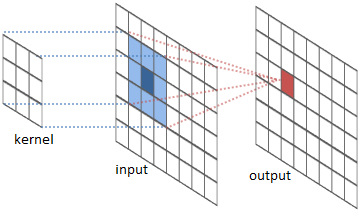
\includegraphics[scale = 0.8]{RiverTrain-ImageConvDiagram}\\
  \caption{RiverTrain-ImageConvDiagram}\label{fig.convolution.RiverTrain-ImageConvDiagram}
\end{figure}

The kernel \href{https://imgbox.com/CIAvIk7p}{slides} to every position of the image
and computes a new pixel as a weighted sum of the pixels it floats over.

\section*{Ref}
\begin{enumerate}
\item \href{http://colah.github.io/posts/2014-07-Understanding-Convolutions/}{Understanding Convolutions}
\item \href{https://www.zhihu.com/question/22298352}{如何通俗易懂地解释卷积?}
\end{enumerate}

